\section{Applications and Experiments}
\label{sec:applications}

We have used the transformation framework to inject different forms of
instrumentation into several programs, both to assess the performance
impact of sampling as well as to show that sampling can offer novel
insights into program (mis)behavior.  We report on our findings here.

\subsection{Sharing the Cost of Assertions}

In conventional usage, C \texttt{assert()} calls are used during
program development but are disabled (``\texttt{-DNDEBUG}'') when the
code ships in order to boost performance.  However, we all know that
shipping release 1.0 does not magically make our code bug-free.
Deployed programs will fail in unanticipated ways, and it would be
helpful to retain some level of assertion checking if the performance
penalty were not excessive.

As an extreme example of assertion-dense code, consider software built
using the \CCured instrumenting translator \cite{POPL_'02*128}.
\CCured analyses programs written in C and attempts to prove,
statically, that most pointer operations are memory safe.  Where this
cannot be done, \CCured inserts dynamic checks to enforce memory
safety at run time.  For purposes of our research, \CCured may be
thought of as a source of highly assertion-dense code.  The individual
assertions are quite small and fast: array bounds checks, testing for
null, etc.  However, in large numbers, their performance impact can be
considerable.  We wish to use random sampling to share this cost
fairly among many users.

We have applied sampling to several benchmarks taken from the
SPECINT95 \cite{SPEC95} and Olden \cite{Carlisle:1996:OPPWDDSDMM}
benchmark suites.  These are the same benchmarked originally examined
by \CCured's designers, but the memory safety bugs they discovered
have been fixed.  Thus all programs run to completion and we are
simply measuring the overhead of performing the dynamic checks.

\subsubsection{Whole-Program Sampling}
\label{sec:ccured:whole}

\begin{table*}[tb]
  \centering
  \begin{tabular}{|l|rrr|rrr|}
    \hline
    & \multicolumn{3}{c|}{\textbf{function counts}} & \multicolumn{3}{c|}{\textbf{average for functions with sites}} \\
    \raisebox{1.5ex}[0pt]{\textbf{benchmark}} & \textbf{total} & \textbf{weightless} & \textbf{has sites} & \textbf{sites} & \textbf{threshold checks} & \textbf{threshold weight} \\
    \hline\hline
    bh & 66 & 14 & 50 & 11.8 & 3.7 & 9.4 \\
bisort & 15 & 3 & 11 & 3.5 & 1.8 & 2.3 \\
em3d & 17 & 5 & 11 & 5.3 & 2.9 & 4.6 \\
health & 18 & 2 & 15 & 5.5 & 2.7 & 3.0 \\
mst & 18 & 6 & 11 & 6.2 & 2.5 & 3.9 \\
perimeter & 11 & 4 & 6 & 6.3 & 2.7 & 1.8 \\
power & 22 & 5 & 17 & 4.9 & 2.7 & 2.7 \\
treeadd & 9 & 2 & 6 & 2.8 & 1.8 & 2.2 \\
tsp & 14 & 5 & 8 & 14.1 & 3.9 & 3.5 \\

    \hline
    compress & 23 & 4 & 18 & 6.3 & 2.6 & 3.7 \\
go & 382 & 12 & 361 & 14.7 & 5.9 & 4.7 \\
ijpeg & 316 & 27 & 272 & 18.5 & 5.0 & 7.3 \\
li & 377 & 16 & 336 & 6.2 & 3.2 & 2.9 \\

    \hline
  \end{tabular}
  \caption{Static metrics for \CCured benchmarks.  Olden benchmarks
    are listed first, followed by SPECINT95.}
  \label{tab:ccured-static}
\end{table*}

\autoref{tab:ccured-static} summarizes static aspects of the sampling
transformation when applied to the entirety of each benchmark.  For
each program, we give the total number of non-library functions and
the number of these which are weightless.  \CCured is a whole-program
analysis, so weightless function identification has the advantage of
being able to examine every function body.  We also count the number
of functions which directly contain at least one instrumentation site.
(What remains are those functions which contain no sites of their own
but which call other functions that do have sites.)

Considering just the functions which directly contain at least one
instrumentation site, \autoref{tab:ccured-static} also presents the
average number of sites per function, the average number of threshold
check points per function, and the average threshold weight for all
such points.  (Note that the product of the last two of these metrics
may exceed the first, as a single instrumentation site may fall under
more than one threshold check point.  This can be seen in the example
in \autoref{fig:code-layout} as well.)  The average site count gives
an impression of how assertion-dense the code is, while the average
threshold weight measures how effective our transformation has been in
amortizing the cost of countdown checks over multiple sites.

\begin{table}
  \centering
  \begin{tabular}{|l|rrrr|}
    \hline
    \rule{0pt}{2.5ex}
    \textbf{benchmark} & $\mathbf{10^{-2}}$ & $\mathbf{10^{-3}}$ & $\mathbf{10^{-4}}$ & $\mathbf{10^{-6}}$ \\
    \hline\hline
    bh & 1.06 & 1.14 & 1.15 & 1.15 \\
bisort & 1.04 & 1.06 & 1.07 & 1.06 \\
em3d & 1.15 & 1.20 & 1.21 & 1.21 \\
health & 1.00 & 1.02 & 1.02 & 1.02 \\
mst & 1.06 & 1.07 & 1.07 & 1.07 \\
perimeter & 0.96 & 0.97 & 0.97 & 0.97 \\
power & 0.97 & 1.00 & 1.00 & 1.00 \\
treeadd & 1.05 & 1.05 & 1.05 & 1.05 \\
tsp & 1.02 & 1.02 & 1.02 & 1.02 \\

    \hline
    compress & 1.32 & 1.38 & 1.39 & 1.39 \\
go & 0.83 & 0.97 & 1.00 & 1.00 \\
ijpeg & 1.24 & 1.32 & 1.34 & 1.34 \\
li & 1.07 & 1.16 & 1.16 & 1.19 \\

    \hline
  \end{tabular}
  \caption{Relative speedup of various sampling rates versus always checking}
  \label{tab:ccured-density}
\end{table}

\autoref{tab:ccured-density} shows the performance effect of various
sampling densities.  We take the running time of standard \CCured code
as the baseline.  We report the speedup ($>1$) or slowdown ($<1$)
relative to this baseline when sampling at various densities.  All
benchmarks were compiled using \texttt{gcc} 2.96 using standard
optimization (\texttt{-O2}).  Times were collected on a 550 MHz
Pentium III Linux machine with two gigabytes of RAM.  Reported
speedups represent the average of four runs; each run used a different
pre-generated bank of 1024 geometrically distributed random
countdowns.

Even at a fairly high sampling density of 1/100, more than two thirds
of our benchmarks run faster then they would if all checks were
performed.  Because each single check is so small and fast, this
suggests that we have largely been successful in amortizing our
sampling overhead.  We are, in a sense, hiding the sampling overhead
in the time that would otherwise have been taken to run 99/100 checks.
The most dramatic speedups are seen in \texttt{ijpeg} (24\% faster)
and \texttt{compress} (32\%) faster.  On the other hand, three of the
benchmarks do run slower, with \texttt{go} showing the largest
penalty.  In these cases, the time recovered by skipping 99/100 checks
is not enough to mask the added overhead of the sampling
infrastructure.

As we reduce the sampling density to 1/1,000, \texttt{power} reaches a
balance point of no measurable speedup or slowdown, while
\texttt{perimeter} remains a stubborn 3\% slower.  The \texttt{health}
benchmark crosses over and is now slightly faster with sampling.
Other benchmarks, which already showed speedups at 1/100, either
retain their position (\texttt{treeadd} and \texttt{tsp}) or show
additional boots, with \texttt{compress} reaching an overall 38\%
speedup versus standard \CCured.  Further reducing the sampling
density to 1/10,000 shows little change, and by the time we reach
1/1,000,000 it is clear that we have reached a performance ceiling.
One benchmark continues to run slower than standard \CCured; two run
at the same speed; the remaining ten run 2\% - 39\% faster.

\subsubsection{Single-Function Sampling}

In an effort to better understand the sources of overhead, we have
performed additional experiments in which only a single function is
instrumented at a time.  This also approximates a more realistic
approach to managing code size.  The fully instrumented executables
from \autoref{sec:ccured:whole} range from 2\%-76\% larger than their
non-sampling counterparts.  When only a single function is
instrumented, code expansion is small enough to not be a concern.

A fully deployed system might use dynamic instrumentation to randomly
instrument a single selected function \textit{du jour}.  For the
present research, we build one executable for each site-containing
function as counted in \autoref{tab:ccured-static}.  All sites in
other functions are removed.  This, in turn, allows us to discover
many more weightless functions: any function which cannot transitively
call the one function being instrumented is weightless.  Thus, a suite
of single-function sampling executables may perform better, over all,
than a single executable with sampling in all functions.

\begin{figure}
  \centering
  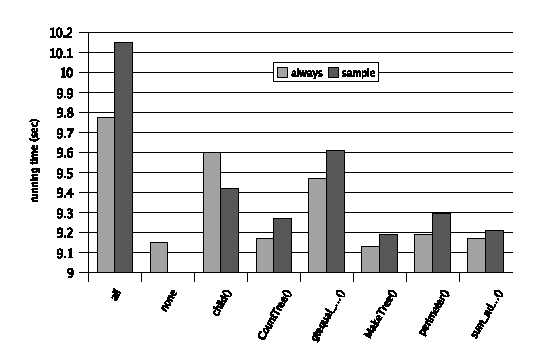
\includegraphics[width=\columnwidth]{applications/perimeter}
  \caption{\texttt{perimeter} running times with single-function
    instrumentation}
  \label{fig:ccured-perimeter}
\end{figure}

In the interest of space, we report only on \texttt{perimeter}: the
stubborn worst performer from the preceding experiment.  This
benchmark's small function count also makes overall results easier to
visualize.  \autoref{fig:ccured-perimeter} shows absolute running
times in seconds, with 1/100 sampling.  The two leftmost ``all'' bars
represent instrumenting all functions, either with checks always done
or with checks sampled.  The solo ``none'' bar represents the extreme
limit of performance: all instrumentation statically removed from all
functions.  No instrumentation scheme, with or without sampling, can
run faster than this.  The remaining bars show the running time for
each site-containing function, with that function's sites either
checked always or sampled 1/100.

Note that the vertical baseline is nine seconds, not zero, which
magnifies fairly small differences: the two leftmost bars differ by
only 4\%, the same difference reported in the ``$10^{-2}$'' column for
\texttt{perimeter} in \autoref{tab:ccured-density}.

Among the site-containing functions, \texttt{Child()} gains a small
performance boot from sampling, while the others slow down.  Examining
each of these in turn, we find:

\begin{description}
\item[\texttt{CountTree()} and \texttt{sum\_adjacent()}] each contain
  only a single instrumentation site.  Thus, threshold checks yield no
  amortization benefit and in fact are optimized away.  Furthermore,
  each function is self recursive (four and two times, respectively),
  and each such call incurs countdown export/import overhead.  This
  could be remedied by transforming each function to pass the local
  countdown to itself as an additional parameter on recursive calls.
  
\item[\texttt{gtequal\_adj\_neighbor()}] is singly self recursive, and
  could benefit form a similar transformation.  Threshold checks
  achieve modest amortization with three instrumentation sites.  Note
  that \texttt{perimeter} overall shows the smallest average threshold
  weight in \autoref{tab:ccured-static}.
  
\item[\texttt{MakeTree()} and \texttt{perimeter()}] achieve good
  amortization from their function-entry threshold checks (weights
  twenty four and five, respectively), but subsequently waste time on
  export/import with four self recursive calls.
\end{description}

Countdown export and import around recursive calls is clearly a
problem, but one with a fairly straightforward solution.  It is worth
noting that \texttt{child()}, which does show speedup, is the only
function of these six which is not self recursive.

Benchmarks that are less dominated by recursion suggest additional
areas for improvement.  Recurring trends include:

\begin{itemize}
\item Poor amortization due to lightweight regions in fixed-bound
  loops.  A loop with fixed iteration count $i$ and body weight $w$
  could be treated as an acyclic region of weight $iw$.  This would be
  similar to using loop unrolling to improve instruction scheduling,
  though literal unrolling is not strictly necessary: merely adjusting
  the weight calculation is sufficient.
  
\item Poor amortization due to lightweight regions in loops with
  bounds fixed on entry.  A similar optimization applies, except that
  the effective region weight $iw$ would be computed from $i$ on each
  new entry into the loop.
  
\item Overly conservative identification of weightless functions.
  Calls through function pointers or to externally-defined code are
  assumed to potentially recurse back to the caller.  Points-to
  analyses can improve the former; a checkable \texttt{weightless}
  annotation on function prototypes would resolve the later.
\end{itemize}

When multiple functions are being instrumented, we find another area
for improvement.  Some callees may not be weightless, but can never
cross more than some finite number of sites per call.  The caller of a
finite-weight function can exploit this upper limit, effectively
treating the callee as a cluster of sites of appropriate weight.  Just
as the loop optimizations resemble loop unrolling without the literal
code change, here we exploit a sort of virtual inlining, but of
weights instead of code.

We expect that these and other optimizations will continue to shrink
the sampling overhead, both for single-function as well as
whole-program instrumentation.

\subsection{Statistical Debugging}
\label{sec:applications:mining}

Sampled information about program behavior can be thought of as a
database.  Data mining techniques, then, may reveal important
information about the aggregate behavior of many runs.  Of particular
interest to us is finding and fixing bugs.  We now illustrate how
mining of sampled program behavior can help direct software engineers
to the root cause of difficult bugs.

Because we do not have ready access to thousands of users, we simulate
a large user community by using randomly generated inputs in the
spirit of the Fuzz project~\cite{MKLMMNS95}.  Our selected target is
version 1.06 of the GNU implementation of \texttt{bc}.  We find that
feeding \texttt{bc} nine megabytes of random input causes it to crash
roughly one time in four.  While this would be an unusually high
failure rate for shipping software under normal usage patterns, we
expect that users experiencing crashes will be more likely to opt-in
to a trace reporting system.  Thus, this may be a reasonable ratio to
expect if most crashes and a few non-crashes are reported.

Quick perusal of the stack trace at a typical failure is discouraging.
The crash occurs several frames deep inside the C library's
\texttt{malloc()} function: a sure sign of heap corruption.  Such bugs
are especially pernicious because the actual corruption may have
happened well before the ultimate crash \cite{Eisenstadt1993b}.

We instrument \texttt{bc} to guess and randomly check a large number
of possible invariants.  Our goal is to identify invariants that hold
when the program succeeds, but which are violated when the program
crashes.  We cast an extremely broad net, but with an eye toward
pointer use violations and buffer overruns.  At any direct assignment
to a scalar variable $x$, we identify all other local or global
variables $\{ y_1, y_2, \dots, y_n \}$ which are also in scope and
which have the same type.  We then compare $x$ to each $y_i$, and
update one of three counters depending on whether $x$ was smaller,
equal to, or greater than $y_i$.  A distinct counter triple is
maintained for each $(x, y_i)$ pair at each distinct syntactic
assignment.  We compare pointers to same-typed pointers as well, and
additionally compare each pointer for equality with null.  One
comparison between $x$ and $y_i$, which bumps one of three counters,
is considered to be one instrumentation site subject to random
sampling.

As expected, this gives us a large number of candidate invariants:
13,442 counter triples, or 40,326 counters in all.  Because our
invariant guesses are so crude, the vast majority of these are of no
interest, either because they compare completely unrelated variables
or because they express invariants which behave indistinguishably in
both successful and failed runs.

To find the few invariants that do count, we use \aside{identify and
  describe the particular form of logistic regression we used.}

\aside{Interpretation of logistic regression results.  Statement that
  they direct us to some small region of code in a single function,
  versus 9764 lines of code in all of \texttt{bc}.  Description of
  previously unreported buffer overrun bug found on like 176 of
  \texttt{storage.c}.
  
  Yes, this is rigged.}

\aside{Alice reports:
  
  \begin{quote}
    Well, of the 40296 features (yet another name for ``predictors''),
    only 9056 of them are ever non-zero.  Of the non-zero useful
    features, 955 are constant; 948 of these are constant at 1, 2 at
    2, 1 at 28, 1 at 31, and 3 at 32.  144 of the useful features have
    very small variation, where the value is only different for one or
    two runs.
  \end{quote}

  And once we sample down to 1/100, we have only 2088 columns, so
  things speed up quite a bit.

  Beyond what this does for the regression analysis, this means the
  counts would compress very well.  That's good news for deployed
  users with slow modems.  It's also good news for the server's hard
  drive.}

\aside{While it is uncommon to do an analysis where the number of
  independent variables swamps the number of observations, there is
  some precedent, especially in biology.  For example:

  \begin{itemize}
  \item 81 samples in 3 classes; 4,682 genes \cite{Dudoit:2002:CDM}
  \item 72 samples in 3 classes; 6,817 genes \cite{Dudoit:2002:CDM}
  \item 64 samples in 9 classes; 5,244 genes \cite{Dudoit:2002:CDM}
  \item 1909 cases (42 positive) in 2 classes; 139,351 binary features
    \cite{2002-cheng}
  \end{itemize}
  
  Although the specific techniques vary, these folks (like us) use
  methodologies which assume that the vast majority of predictors are
  actually irrelevant, and you want to pick out the few that actually
  matter.}

\begin{figure}
  \centering
  \small
  \listinginput{152}{applications/more_arrays.c}
  \caption{Source code of suspect \texttt{bc} function
    \texttt{more\_arrays()}}
  \label{fig:bc:more-arrays}
\end{figure}
